\section{Assvengers}

El presidente ha citado a los "assvengers" a un consejo de héroes latinoamericanos, con el fin de  definir lo que van a hacer contra un Hulk naranjado que quiere ponerle aranceles  a toda latinoamérica. La reunión  iba bien hasta que los héroes se lo tomaron personal, lloraron y alegaron, ya que todos estaban en desacuerdo con la decisión del presidente  de incluir  al Lagarto  en su consejo.

\subsection{Procedimiento gráfico (1.3 pt)}

El primero en quejarse fue el Capitán Sur América ya que el lagarto no cree que el nuevo Capitán  sea tan "papucho" como el anterior y lo tiene mal condicionado. Si la función de inestabilidad psicológica del Capi es:

\[ f(x) = \ln{x} + \frac{1}{x-c} \]
\[ f(x) = \ln{x} + \frac{1}{x-0} \]
\[ g(x) = \left|\frac{xf'(x)}{f(x)}\right| \]
\[ Z(x) = 1 \]

\begin{figure}[H]
    \centering
    \begin{subfigure}[b]{\textwidth}
        \centering
        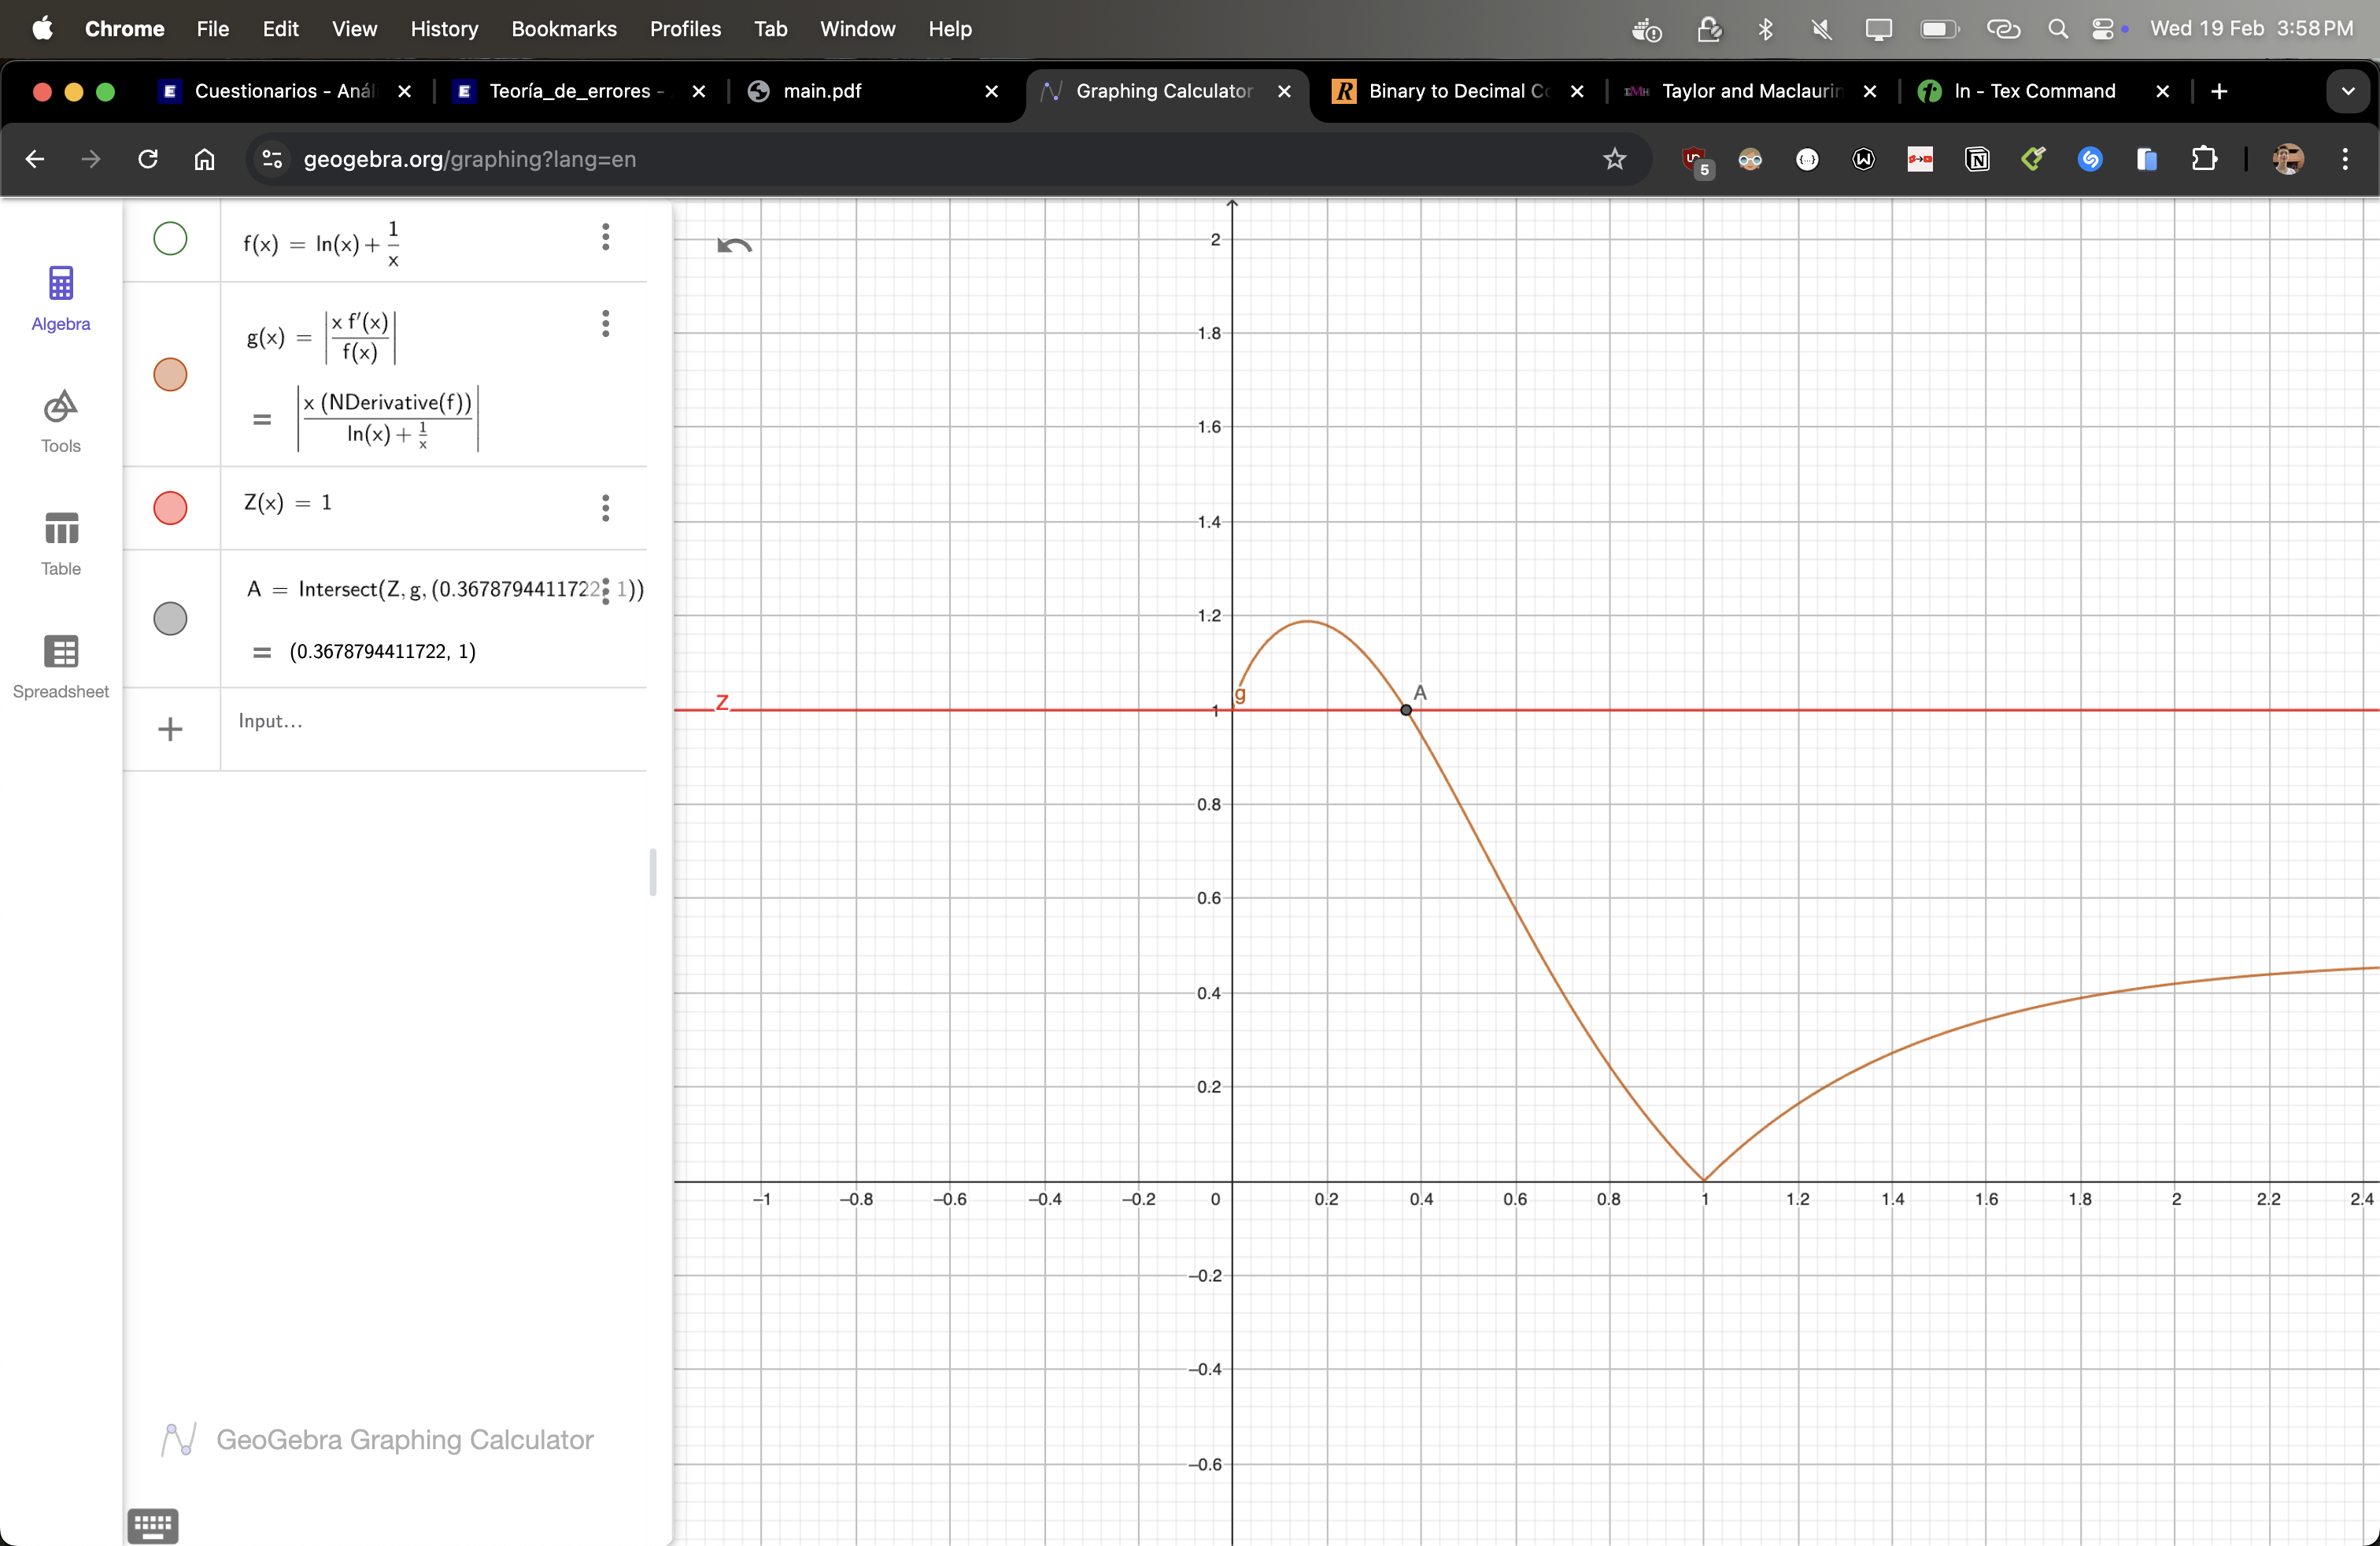
\includegraphics[width=\textwidth]{Figures/0. General/1.1.png}
        \caption{Gráfica g(x) con el intersecto sobre Z(x)}
        \label{fig: Grafica g(x)}
    \end{subfigure}
\end{figure}

De $0$ a el Intersecto $A$ $(0.368, 1)$ la función $g(x)$ (en este caso la función de condición)
es mayor que 1, y de $0.368$ a $\infty$ la función $g(x)$ es menor que 1. Por lo tanto,
la inestabilidad de Capitán Sur América está mal condicionada en el intervalo $[0, 0.368]$.

\subsection{Aproximación de Taylor (1.3 pt)}
El número de condición anterior también representa el mal condicionamiento de toda latinoamérica, y sirve para encontrar los aranceles que nos va a imponer el Hulk naranja, sin embargo, es necesario usar una aproximación de Taylor  de tres términos centrada en 2 para el número de condición . Encuentre la aproximación de Taylor que representa los aranceles.


\subsubsection{Definir la función \(f(x)\) y su derivada}

Del enunciado se ve que
\[
f(x) \;=\; \ln(x) \;+\;\frac{1}{x}.
\]
Por tanto,
\[
f'(x) 
=\frac{d}{dx}\Bigl(\ln(x)+\tfrac{1}{x}\Bigr)
=\frac{1}{x}\;-\;\frac{1}{x^2}
=\frac{x-1}{x^2}.
\]

\subsubsection{Definir la función \(g(x)\)}

Se ha dado que
\[
g(x) 
\;=\;\left|\frac{x\,f'(x)}{f(x)}\right|
\;=\;\frac{x\,f'(x)}{f(x)}
\quad(\text{alrededor de }x=2, \text{es positiva, así que el valor absoluto no altera el signo}).
\]
Sustituyendo \(f'(x)\) y \(f(x)\):

\[
x\,f'(x) \;=\; x \cdot \frac{x-1}{x^2}
\;=\;\frac{x-1}{x},
\]
\[
f(x) \;=\;\ln(x)+\tfrac{1}{x}.
\]
Por lo tanto,
\[
g(x) 
=\frac{\frac{x-1}{x}}{\ln(x) + \tfrac{1}{x}}
=\frac{x-1}{x\,\ln(x) + 1}.
\]

Para simplificar la notación, definamos
\[
G(x)\;=\;\frac{x-1}{\,x\,\ln(x)\;+\;1\,}.
\]
Este \(G(x)\) es la misma \(g(x)\) (sin el valor absoluto), y la expandiremos en serie de Taylor alrededor de \(a=2\).


\subsubsection{Calcular los valores y derivadas en \(x=2\)}

La \textbf{serie de Taylor} de segundo orden (tres términos) centrada en \(x=2\) es

\[
G(x)\;\approx\;G(2)
\;+\;G'(2)\,\bigl(x-2\bigr)
\;+\;\tfrac12\,G''(2)\,\bigl(x-2\bigr)^{2}.
\]

\subsubsection{Valor de \(G(2)\)}

\[
G(2)
=\frac{2-1}{\,2\,\ln(2)+1\,}
=\frac{1}{\,2\,\ln(2)+1\,}.
\]
Nótese que \(\ln(2)\approx 0.693147\), por lo que  
\(\,2\,\ln(2)\approx 1.386294\) y \(2\ln(2)+1\approx 2.386294\).  
Así,
\[
G(2)\approx \frac{1}{2.386294}\;\approx\;0.419.
\]

\subsubsection{Primera derivada \(G'(x)\) y su valor en \(x=2\)}

Sea \(u(x)=x-1\) y \(v(x)=x\,\ln(x)+1\). Entonces 
\[
G(x)=\frac{u(x)}{v(x)}.
\]
La regla del cociente da:
\[
G'(x)
=\frac{u'(x)\,v(x)-u(x)\,v'(x)}{\bigl[v(x)\bigr]^2}.
\]

\begin{itemize}
    \item \(u'(x)=1.\)  
    \item \(v'(x)=\tfrac{d}{dx}\bigl[x\ln(x)\bigr]+0=\ln(x)+1.\)
\end{itemize}

Por tanto,
\[
G'(x)
=\frac{\;[1]\,[\,x\ln(x)+1\,]\;-\;[x-1]\,[\ln(x)+1]}{[\,x\ln(x)+1\,]^2}
=\frac{x\ln(x)+1 - (x-1)(\ln(x)+1)}{[\,x\ln(x)+1\,]^2}.
\]
La parte superior se simplifica:
\[
x\ln(x)+1 
-\bigl[(x-1)\ln(x)+(x-1)\bigr]
= x\ln(x)+1 - \bigl[x\ln(x)-\ln(x)+x-1\bigr]
\]
\[
=\;x\ln(x)+1 
- x\ln(x) + \ln(x) - x + 1
=\;2\;+\;\ln(x)\;-\;x.
\]
Por tanto,
\[
G'(x)=\frac{\,2 + \ln(x) - x\,}{\bigl[x\ln(x)+1\bigr]^2}.
\]
Evaluando en \(x=2\):

\[
G'(2)
=\frac{\,2 + \ln(2) - 2\,}{\bigl[\,2\ln(2)+1\,\bigr]^2}
=\frac{\ln(2)}{\bigl[\,2\ln(2)+1\,\bigr]^2}.
\]
Con \(\ln(2)\approx 0.693147\) y \(2\ln(2)+1\approx 2.386294\),  
\(\bigl[2\ln(2)+1\bigr]^2\approx 5.691,\)  
por lo que 
\[
G'(2)\approx \frac{0.693147}{5.691}\;\approx\;0.122.
\]

\subsubsection{Segunda derivada \(G''(x)\) y su valor en \(x=2\)}

Aunque es más laborioso, se procede de la misma manera (regla del cociente con \(p(x)=2+\ln(x)-x\) y \(q(x)=[x\ln(x)+1]^2\)), o usando la fórmula anterior:

\[
G'(x)=\frac{p(x)}{q(x)}, 
\quad
p(x)=2+\ln(x)-x,\quad
q(x)=[\,x\ln(x)+1\,]^2.
\]
\[
G''(x)=\frac{p'(x)\,q(x)-p(x)\,q'(x)}{[\,q(x)\,]^2}.
\]

\begin{itemize}
    \item \(p'(x)=\tfrac{d}{dx}[2+\ln(x)-x]=\tfrac{1}{x}-1.\)
    \item \(q'(x)=2\,[\,x\ln(x)+1\,]\cdot(\ln(x)+1)\)  (por regla de la cadena).
\end{itemize}

Finalmente se evalúa todo en \(x=2\). El resultado numérico aproximado es

\[
G''(2)\;\approx\;-0.261.
\]

\subsubsection{Serie de Taylor de tres términos alrededor de \(x=2\)}

La \textbf{aproximación de Taylor} de segundo orden (tres términos) es:

\[
G(x)\;\approx\;G(2)
\;+\;G'(2)\,\bigl(x-2\bigr)
\;+\;\tfrac12\,G''(2)\,\bigl(x-2\bigr)^{2}.
\]
Con los valores numéricos ya calculados:

\begin{itemize}
    \item \(G(2)\approx 0.419.\)
    \item \(G'(2)\approx 0.122.\)
    \item \(G''(2)\approx -0.261.\)
\end{itemize}

\begin{figure}[H]
    \centering
    \begin{subfigure}[b]{\textwidth}
        \centering
        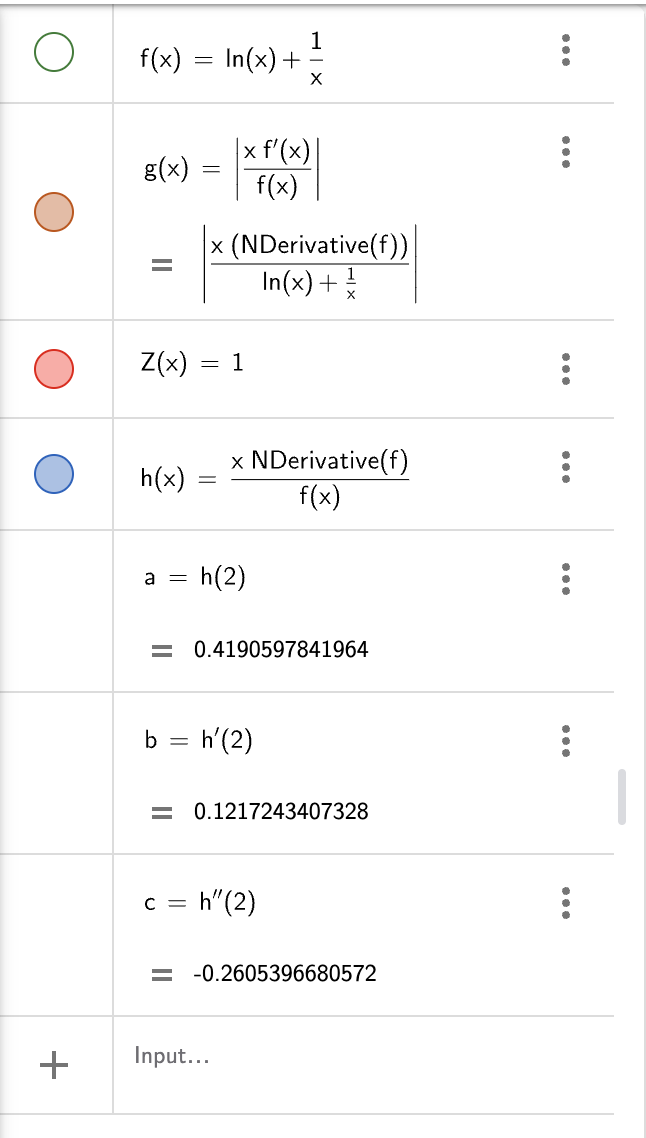
\includegraphics[width=0.4\textwidth]{Figures/0. General/1.2.png}
        \caption{Comprobación de valores $G(2)$, $G'(2)$ y $G''(2)$ en Geogebra}
        \label{fig: Comprobacion en Geogebra}
    \end{subfigure}
\end{figure}

Por lo tanto,

\[
\boxed{
g(x)\;\approx\;0.419 
\;+\;0.122\,(x-2)
\;-\;0.130\,(x-2)^{2}.
}
\]
donde \(\,-0.130\,\) proviene de \(\tfrac12\,\bigl(-0.261\bigr)\).  

En forma simbólica exacta (sin redondeos), se puede dejar:
\[
g(2) \;=\;\frac{1}{\,2\ln(2)+1\,},\quad
g'(2)\;=\;\frac{\ln(2)}{\bigl[\,2\ln(2)+1\,\bigr]^2},\quad
g''(2)\;=\;\frac{\text{(expresión en }\ln(2)\text{)}}{\bigl[\,2\ln(2)+1\,\bigr]^4}.
\]

\subsection{Exactitud (1.4 pt)}

Otro momento importante  de la reunión  fue cuando "Novelaman" le confesó al presidente  su amor y decidió  pagar los aranceles anteriores como regalo de San Valentín. En principio él necesita saber cuánto representan estos aranceles cuando la aproximación de Taylor se evalúa en dos de los valores del intervalo de mal condicionamiento (ejercicio 1). Para estar seguro que no lo están robando, Novelaman calcula también los aranceles con el número de condición verdadero, pero no obtiene los mismos resultados, así que afirma que el Lagarto se está robando la platica.  Calcule usted las exactitudes que tienen dos valores pertenecientes al intervalo de mal condicionamiento del ejercicio 1 y explique a Novelaman, porque le dan diferentes las exactitudes.  (Puede usar cualquier valor de su elección en el intervalo de mal condicionamieto) Entregue su procedimiento y explicación.


\begin{itemize}
    \item \textbf{Fórmula exacta} de \(g(x)\) (sin valor absoluto para simplificar la comparación de signos):  
    \[
        g_{\text{exact}}(x) \;=\; \frac{x-1}{\,x\,\ln(x)\;+\;1\,}.
        \]
        \textbf{(Corresponde a \(\frac{x\,f'(x)}{f(x)}\) con \(f(x)=\ln(x)+\frac{1}{x}\).)}
        
    \item \textbf{Aproximación de Taylor} de segundo orden (3 términos) centrada en \(x=2\), que llamamos \(g_{\text{approx}}(x)\):
    
       \[
       g_{\text{approx}}(x) 
       \;\approx\; 0.419 
         \;+\;0.122\,\bigl(x-2\bigr)
         \;-\;0.130\,\bigl(x-2\bigr)^{2}.
       \]
       Estos valores numéricos (\(0.419\), \(0.122\), \(-0.130\)) provienen de evaluar \(g(2)\), \(g'(2)\) y \(\tfrac12\,g''(2)\).
    \item \textbf{Error relativo} (una definición frecuente)  
    \[
    \text{Error relativo}(x)
    \;=\;\frac{\bigl|\,g_{\text{exact}}(x)\;-\;g_{\text{approx}}(x)\bigr|}{\bigl|\,g_{\text{exact}}(x)\bigr|}.
    \]
    Entonces la “exactitud” (en \%) a veces se expresa como  
    \[
    \text{Exactitud}(x)
    \;=\;100\%\times \Bigl(1 - \text{Error relativo}(x)\Bigr).
    \]
    \end{itemize}


\subsubsection{Elección de valores en \([0,\,0.368]\)}

Tomemos por ejemplo:
\begin{itemize}
    \item \(x_1 = 0.30\).  
    \item \(x_2 = 0.35\).
\end{itemize} 

Ambos están dentro del intervalo “mal condicionado” identificado en el ejercicio 1 (\([0,\,0.368]\)).

\subsubsection{2.1. Cálculo en \(x=0.30\)}

1. \textbf{Valor exacto} 
   \[
   g_{\text{exact}}(0.30) 
   \;=\; \frac{0.30 - 1}{\,0.30\,\ln(0.30)\;+\;1\,}.
   \]  
   Observemos que \(\ln(0.30)\approx -1.2039728\). Entonces  
   \[
   0.30 \,\ln(0.30)\;\approx\;-0.3611918,
   \quad
   [\,0.30\,\ln(0.30)+1\,]\;\approx\;1 - 0.3611918\;=\;0.6388082.
   \]  
   Numerador: \(0.30 - 1 = -0.70\).  
   \[
   g_{\text{exact}}(0.30)
   \;\approx\;\frac{-0.70}{0.6388082}
   \;\approx\;-1.0956.
   \]

2. \textbf{Valor aproximado (Taylor)}  
   \[
   g_{\text{approx}}(0.30)
   \;=\;0.419 \;+\;0.122\,(0.30-2)\;-\;0.130\,(0.30-2)^{2}.
   \]
   \begin{itemize}
         \item \( (0.30 - 2) = -1.70\).  
         \item \( (0.30 - 2)^2 = 2.89\).
         
    \end{itemize}
   Entonces:  
   \[
   g_{\text{approx}}(0.30)
   \approx 0.419 
         \;+\;0.122\,(-1.70)
         \;-\;0.130\,(2.89).
   \]
   \[
   = 0.419 
     \;-\;0.2074
     \;-\;0.3757
   \;=\;-0.1641 \;\text{(aprox.)}
   \]

3. \textbf{Error relativo y exactitud} 
   \[
   \text{Error absoluto} 
   \;=\;\bigl|-1.0956 - (-0.1641)\bigr|
   \;=\;0.9315.
   \]
   \[
   \text{Error relativo} 
   = \frac{0.9315}{|\,-1.0956\,|}
   \approx \frac{0.9315}{1.0956}
   \;\approx\;0.85 \;=\;85\%.
   \]
   Por tanto,  
   \[
   \text{Exactitud}
   \;=\;100\%\times(1 - 0.85)
   \;=\;15\%.
   \]

\subsubsection{2.2. Cálculo en \(x=0.35\)}

1. \textbf{Valor exacto} 
   \[
   g_{\text{exact}}(0.35)
   \;=\; \frac{0.35 - 1}{\,0.35\,\ln(0.35)+1\,}.
   \]
   \(\ln(0.35)\approx -1.0498221\). Entonces  
   \[
   0.35\,\ln(0.35)\approx -0.3674377,
   \quad
   [\,0.35\,\ln(0.35)+1\,]\approx 1 - 0.3674377 = 0.6325623.
   \]
   Numerador: \(0.35 - 1 = -0.65.\)  
   \[
   g_{\text{exact}}(0.35)
   \approx \frac{-0.65}{0.6325623}
   \;\approx\;-1.028.
   \]

2. \textbf{Valor aproximado (Taylor)}
   \[
   g_{\text{approx}}(0.35)
   = 0.419 
     \;+\;0.122\,(0.35-2)
     \;-\;0.130\,(0.35-2)^{2}.
   \]
   \begin{itemize}

   \item \((0.35 - 2) = -1.65.\)
   \item \((0.35 - 2)^2 = 2.7225.\)  
   
    \end{itemize}
   \[
   g_{\text{approx}}(0.35)
   \approx 0.419 
     \;+\;0.122\,(-1.65)
     \;-\;0.130\,(2.7225).
   \]
   \[
   = 0.419 
     \;-\;0.2013
     \;-\;0.3539
   = -0.1362 \;\text{(aprox.)}
   \]

3. \textbf{Error relativo y exactitud}
   \[
   \text{Error absoluto} 
   = \bigl|-1.028 - (-0.1362)\bigr|
   = 0.8918.
   \]
   \[
   \text{Error relativo}
   = \frac{0.8918}{1.028}
   \;\approx\;0.867 \;=\;86.7\%.
   \]
   \[
   \text{Exactitud}
   = 100\%\times (1 - 0.867)
   = 13.3\%.
   \]

\subsubsection{¿Por qué difieren tanto?}

Observamos que la aproximación de Taylor se \textbf{centra en \(x=2\)}, pero estamos evaluando en valores muy \textbf{lejanos} a 2 (\(0.30\) y \(0.35\)). El polinomio de Taylor de pocos términos (solo hasta segundo orden) no es fiable cuando nos alejamos tanto del punto de expansión, sobre todo si la función \(g(x)\) varía drásticamente (y \(\ln(x)\) se hace negativa, etc.).\\

En otras palabras, \textbf{no es que el Lagarto “esté robando la plata”}, sino que la \textbf{aproximación de Taylor} (hecha en \(x=2\)) sufre un \textbf{error de truncamiento muy grande} para valores de \(x\) cercanos a 0 (o muy por debajo de 2). Eso explica por qué \(g_{\text{exact}}(x)\) y \(g_{\text{approx}}(x)\) difieren tanto en el intervalo mal condicionado \([0,\,0.368]\).  

